% -----------
% SETUP
% -----------
\documentclass{physics_article_B}
\title{Mechanical Vibrations of Droplets in Fluidic Systems}
\mytitle{Mechanical Vibrations of Droplets in Fluidic Systems}
\myname{Dominic Coy \& Oliver Gordon}
\studentid{4227789 \& 4224942}
\date{Due Date: 1 June 2018}
\setlength{\bibsep}{10pt plus 0.3ex}
\begin{document}
    
% ----------------------
% COVERSHEET
% ----------------------
\pagenumbering{roman} 
\setcounter{page}{0}
\includepdf[scale=1,offset=1.9mm -4.4mm]{CoverFin.pdf}
\newpage
\newpage
\thispagestyle{empty}
\mbox{}
\newpage

% ----------------------
% ABSTRACT
% ----------------------
\pagenumbering{roman} 
\setcounter{page}{1}
\begin{abstract}
    \large{\textit{The aim of this project was to develop an automated system to analyse the rheological properties of single fluidic droplets suspended in mineral oil. This was accomplished through the creation of a flow system to create, suspend and transport spherical droplets in mineral oil. Real-time computer vision was then used to determine the radius of the droplet to an accuracy of $\pm$ 0.03 mm. It was found that oscillations could then be induced using either a DC electric field or a copper obstruction. After observing these oscillations using a laser and photodiode, frequency analysis was then performed. For distilled water, it was found that surface tension, $\gamma$ = 21.54 $\pm$ 17.57 mNm$^{-1}$ and viscosity, $\eta$ = 11.77 $\pm$ 6.63 x 10$^{-4}$ Nm$^{2}$s$^{-1}$. Although these values were only within an order of magnitude of expected values, this can be explained by a combination of incomplete theory and the short length of time that oscillations were detected for. From the foundations laid in this project, it is evident that the vibration of droplets in automated high-throughput systems could potentially be a key method of rheology in the future.}}
\end{abstract}

\begin{center}
\vspace{0.4cm}
{\Large\bf{Acknowledgements}} \\
\addcontentsline{toc}{section}{Acknowledgements}
\end{center}

\begin{changemargin}{1cm}{1cm} 
\textit{We would like to acknowledge the many people who helped us over the course of the project. In particular, we would like to acknowledge our project supervisor James Sharp, the laboratory technicians Matthew Young and Paul Munday, and Florian Enner from Hebirobotics for their continued assistance. We would also like to thank Thomas Li for briefly providing to us the use of his high-speed camera.}


\end{changemargin}
\vspace*{\fill}

% ----------------------
% CONTENTS
% ----------------------
%\vspace{4cm}
\newpage
\tableofcontents

\setlength{\parskip}{8pt}  
% ----------------------
% INTRODUCTION
% ----------------------
\newpage
\pagenumbering{arabic} 
\setcounter{page}{1}

\section{Introduction\label{sect:intro}}

    Simultaneously measuring the rheological properties of fluids, such as viscosity and surface tension, has, in the past, been accomplished with rheometers\cite{harrold2} or drop volume techniques\cite{miller1992}. Besides being a key method for identifying materials, understanding the rheology of a material makes it possible to alter its behaviour in a controlled fashion. However, these existing methods are not particularly viable when analysing rare or expensive fluids, such as blood droplets in forensics, as they require large volumes of fluid. When only a few millilitres of fluid is available, the most promising analysis method is to induce oscillations in small droplets\cite{harrold}, and analyse how these oscillations refract a laser through the droplet using a photodiode. Other applications of this vibrational method and supporting theory include monitoring inkjet printing performance\cite{Martin2008}, simulating the crustal deformation of planets\cite{vukasinovic}, and studying energy relaxation in stars\cite{vukasinovic}.
    
    Early experiments using droplets in rheology were based on theoretical models developed by Rayleigh\cite{rayleigh} and Chandrasekhar\cite{chandrasekhar2} who showed that, by using simple equations, the vibrational frequencies of droplets were related to the viscosity and surface tension of a viscous sphere of fluid. In 2014, Temperton et al. claimed to be the first to present a combined theoretical and experimental study of simple Newtonian fluids, such as water\cite{temperton}. This approach was later extended by multiple authors who demonstrated that, provided surface tension is already known, this technique could be used to extract frequency dependent physical properties of viscoelastic droplets, such as blood\cite{egry}. 
    
    Although multiple authors have demonstrated the viability of manual testing\cite{benmore,Meier2000,Egry1998}, this is not ideal. As such, the aim of this project was to develop a system to automate this process. This involved building a high-throughput system (an automated system allowing the large scale repetition of the experiment) to consistently create and transport spherical droplets suspended in oil. The size of the droplets were also calculated using real time computer vision, which is the process by which a computer can see and react to images. After oscillating the droplets, they were then analysed with a laser and photodiode to determine their rheological properties.
    
    In the future, the ability to track the properties of a fluid in real time using a high-throughput system, first considered by Harrold et al. in 2016\cite{harrold}, could be applied to lab-on-a-chip systems, such as inexpensive, reliable tests\cite{yager} for medical diagnosis. Furthermore, droplets containing mixed fluids could also be investigated along with simultaneously measuring the interfacial tension between both the droplets and the carrier fluid\cite{Backholm2017}. This project aimed to demonstrate the viability of, and build upon, such a system.
    
    In this paper, the history of the field is first discussed, along with the associated theory. Next, the techniques used to locate the droplets and determine their size are covered. The four different methods used to attempt to induce oscillations are debated, followed by an explanation of how the system was automated. The validity of this system is demonstrated using distilled water, before discussing the results of the project and their implications. Finally, future improvements that could be made to the project and future directions to take the research are discussed.

% ----------------------
% Literature Review
% ----------------------
\newpage\section{Literature Review\label{sect:lit}}

    Building on the work done by Rayleigh in 1879, which related the frequency of oscillation of fluidic jets with their area and pressure\cite{rayleigh}, in 1933 Lamb et al.\cite{lamb} derived an expression for the oscillation frequency of inviscid (negligible viscosity) droplets in an inviscid fluid. They also derived approximate expressions for the rate of damping of oscillations in a viscous droplet in an inviscid fluid and for the oscillations of a bubble of gas in a low viscosity liquid. In their derivations, the velocity fields found for small oscillations of an inviscid fluid were used to estimate the rate of viscous dissipation (the rate that shear forces turn work done by a fluid on adjacent layers into heat) in a droplet with small viscosity\cite{lamb}. Then, in 1960, Reid et al. experimentally demonstrated the oscillations of a viscous droplet in a low-density gas or a vacuum\cite{reid}. His experiment and analysis were later summarised in the book Hydrodynamics and Hydrodynamic Stability by Chandrasekhar in 1961\cite{chandrasekhar}. In 1965, Velentine et al. used the same methods as Lamb et al. to derive expressions for the damping rate of oscillations when a low viscosity droplet was submerged in a low viscosity fluid\cite{velentine}. In 1968, Miller et al.\cite{miller} derived equations for the decay time and oscillatory frequencies of oscillating viscous droplets immersed in a viscous fluid. These could also be applied when the interface between the two fluids possessed elastic and viscous properties of its own. They also derived equations for the rate of damping of oscillations and frequency for specific cases including when the interface between the two fluids was free or is inextensible.
    
    Since then, experiments have focused on a variety of droplet shapes. Two of the three common droplet shapes are sessile (lying on a surface)\cite{vukasinovic, Backholm2017, Temperton2012} and pendant (teardrop-shaped and suspended off a surface such as a needle)\cite{Temperton2012}. Despite the relative experimental ease of investigating these suspended droplets, damping interactions and droplet shape can be influenced by the suspension surface\cite{Sharp2011}. This alters the vibrational spectra of the droplets, producing errors yet to be fully rectified\cite{harrold}. Despite this, many authors limit such experiments to sessile droplets lying on a single surface\cite{Sharp2011}, leading to differing results. The influence of the suspension surface can be partly avoided by using either superhydrophobic or superamphiphobic surfaces\cite{harrold}. This is because the droplets would take on a more spherical shape and could be described with similar equations to levitated droplets derived by Miller et al. There is, therefore, an impetus to find a reliable method to create fully spherical droplets to remove the influence of the suspension surface altogether.
    
    Much of the initial research involving spherical droplets was driven by the ambition to study containerless crystallisation of pure liquids in microgravity\cite{wilkes}. However, much of the current research has been focused on the determination of the rheological properties of the droplets\cite{harrold2,benmore,capillary}. Although it is possible to investigate large spherical droplets by performing the experiment in low gravity (as done in 1979\cite{holt} on Space Shuttle Columbia), this is impractical in this project. Therefore, a wide variety of alternative methods for levitating droplets, other than using microgravity, have been considered. Methods previously used to levitate the droplets include magnetic\cite{temperton, hill}, electrostatic\cite{mugele, wong}, acoustic\cite{trinh, Yarin1998} and aerodynamic\cite{benmore}. Alternatively, McHale et al. demonstrated the feasibility of determining rheological properties of levitated droplets by using vibrating liquid marbles (droplets stabilised by the adsorption of small particles). However, they found that the small particles dominated the droplet's physical properties and so the application of this approach was limited\cite{mchale}. Therefore, there is a great interest in analysing droplets suspended within another fluid as the droplets do not need to be stabilised by the adsorption of small particles and hence, act like levitated droplets. 
    
    \newpage One of the main advantages of suspending a droplet within another fluid over other methods of levitation is that of a lower mass loss. During an experiment, mass will be lost as the droplet evaporates over time. When suspended within another fluid, this has been shown\cite{harrold2} to be 2 - 4\%, which is significantly lower than for other methods which see over 10\% mass loss. However, to the best of our knowledge, no author has mathematically modelled this mass loss and taken it into account. Furthermore, the way in which mass is calculated is also very basic; the droplet is weighed before and after an experiment by comparing the mass of a syringe or paper towel both with and without the droplet\cite{temperton}. These methods do not take into account leftover residue, and in the case of paper towels are destructive. Additionally, other methods of levitation require placing droplets by hand, which is a slow process. Therefore, there is a significant impetus to develop a high throughput system allowing multiple droplets, suspended within another fluid, to be quickly analysed.

\section{Theory\label{sect:theory}}

    Following on from previous work\cite{temperton}, the major assumption was taken that the droplets analysed in this project were perfectly spherical. This was because the lowest energy state (and therefore shape) of a droplet was influenced by its surface tension, $\gamma$, and gravitational interactions, $g_{eff}$. $\gamma$ made the droplet spherical, while $g_{eff}$ distorted it. Because these two interactions opposed each other, there existed a critical droplet radius at which its shape would change from being spherical to distorted. This was the capillary length, $l_{cap}$, and was defined by the equation\cite{temperton},
        
        \begin{equation} 
        \label{eq:lcap}
            l_{cap} = \sqrt{\frac{\gamma }{\rho g_{eff} }}, 
        \end{equation}
    
    where $\rho$ was the density of the droplet. It was therefore assumed that a droplet was spherical if it has a radius, $R$, smaller than its capillary length $l_{cap}$. However, as $l_{cap}$ would not always be known for unknown droplets, it was imperative that droplets were kept as small as possible during the project. 

    As the droplet had an equilibrium state, it would undergo shape oscillations when a small perturbation was applied\cite{oscillate}. If this perturbation was in the form of an impulse, the surface of the droplet would be driven at all frequencies. This was because Fourier transforming a delta function yields a constant amplitude at all frequencies. The oscillations not at the resonant frequency were damped, leaving only the vibrations at the resonant frequency of the droplet with a non-zero amplitude. For optimal results, it has been shown that any applied impulse must be long enough to give sufficient time to perturb the drop, but short enough to still be an impulse and not drive the droplet at a particular frequency\cite{temperton}. Furthermore, the amplitude of oscillations must be kept to under 0.1$R$, following work from Becker et al. who found that above this limit oscillations become non-linear, causing the simple equations used here to fail\cite{becker}.
    
    These oscillations decayed exponentially, giving a time dependent signal such as the one shown in Figure \ref{fig:temperton:signal}\cite{temperton}. The power spectral density was then obtained by Fourier transforming this signal and is shown in Figure \ref{fig:temperton:PD}. The remaining resonant frequencies corresponded to different modes, $n$, of oscillation. The $n=1$ mode corresponded to oscillations of the droplet's centre of mass\cite{miller}, while the $n\geq2$ modes corresponded to the surface oscillations of interest in this project. The corresponding frequency, $f_n$, and full-width-half-maximum, $\Delta f_n$, were then extracted from the power spectral density. 

        \begin{figure}[H]
            \centering
                \begin{subfigure}[b]{0.48\textwidth}\hspace*{-0.2cm}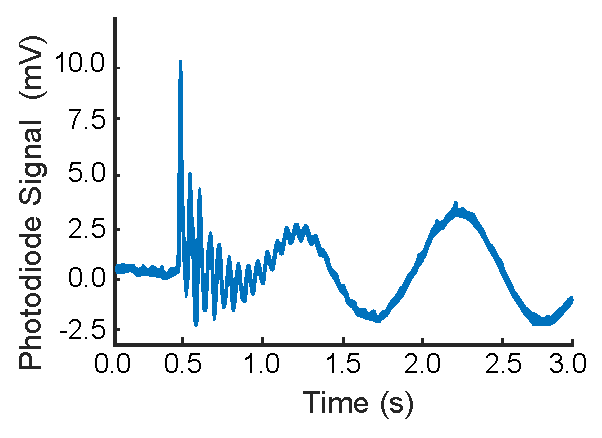
\includegraphics[width=\textwidth]{Figures/TempertonSignal.eps}
                    \caption{Photodiode Signal}
                    \label{fig:temperton:signal}
                \end{subfigure}\hspace{3pt}
                \begin{subfigure}[b]{0.48\textwidth}\hspace*{0.2cm}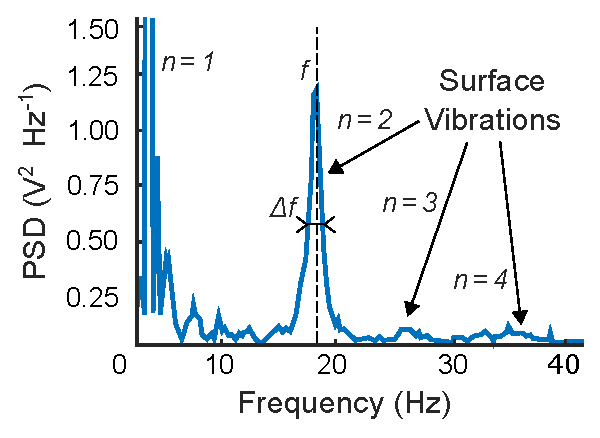
\includegraphics[width=\textwidth]{Figures/TempertonSignalPD.eps}
                    \caption{Fourier transform}
                    \label{fig:temperton:PD}
                \end{subfigure}
            \caption{Figure to demonstrate the time dependent signal produced when oscillating a droplet of water with an impulse (a), and its resulting Fourier transform (b). The resonant vibrations on the surface of the droplet can be seen in (a) as the initial, rapidly oscillating components of the signal. These correspond to multiple modes, $n$, of oscillation in (b). The frequency, $f$, and full-width-half-maximum, $\Delta f$, can then be used to determine the rheological properties of the droplet. Adapted from Temperton et. al.\cite{temperton}}\label{fig:temperton}
        \end{figure}

    The surface tension, $\gamma$, and viscosity, $\eta$, of the fluid were then calculated using the equations,
 
        \begin{equation} 
        \label{eq:SurfaceTension}
            \gamma = \frac{4\rho R^{2}}{\pi n^{2}}(\Delta f^{2} + f^{2}),
        \end{equation}
        
        \begin{equation} 
        \label{eq:Viscosity}
            \eta = \frac{\pi \rho \Delta f R^{2}}{n^{2}}.
        \end{equation}

    For pure water in air, it was expected that\cite{expected1} $\gamma$ = 72.80 mNm$^{-1}$ and\cite{expected2} $\eta$ = 8.94 x 10$^{-4}$ Nm$^{2}$s$^{-1}$. However, these values and equations did not perfectly apply to the water in oil used in this project. In the absence of a complete theory these results served as a guideline to the expected values. 
    
    Furthermore, Equations \ref{eq:SurfaceTension} and \ref{eq:Viscosity} were only valid for simple Newtonian droplets such as water and glycerol. For viscoelastic droplets such as amorphous polymers, biopolymers, metals at very high temperatures, or bitumen materials, there has yet to be a complete analysis of droplets without prior knowledge of their surface tension. Further, these equations assume that the volume of the droplet remains constant. As such, only liquids can be analysed as they are incompressible.
    
    To determine $R$, checkerboards of known dimensions were used to map the pixels on a screen to real world space. Because cameras have no depth-perception, this required the assumption that the object of interest was in the same plane as the checkerboard\cite{CameraCalibration}. Once the height and width of a spherical droplet, $D_x$ and $D_y$ respectively, was found in an image containing a checkerboard, $R$ was calculated with the simple trigonometry shown in Equation \ref{eq:radii},
            
        \begin{equation}\label{eq:radii}
            R = \sqrt{\Big(\frac{D_x}{2}\Big)^2 + \Big(\frac{D_y}{2}\Big)^2}.
        \end{equation}

% ----------------------
% Method
% ----------------------
\section{Methods\label{sect:method}}

    \subsection{Slide \& Fluid Loop\label{sect:method:slide}}
    
        To interrogate liquids of interest, a clean test environment had to be created. This was accomplished by first creating a plastic mould with a 2 mm diameter tunnel inside. This ensured that all droplets were well below the 2.7 mm capillary length of water\cite{capillary}. The mould was then filled with polydimethylsiloxane (PDMS), glued on a glass slide and cured. A 1 mm port was also created on the top side of the slide which was subsequently used to inject fluids of interest. This smaller diameter was chosen as the higher pressure it created prevented oil from flowing backwards, and further droplets being unintentionally created.
        
        Three 2 mm diameter capillary tubes, with a 1 mm internal diameter, were then attached to these ports, before sealing all leaks with flowable silicon. This setup is demonstrated in Figure \ref{fig:slide}. Manufacturing a perfectly sealed PDMS slide with smooth tunnels was a slow process due to the long drying time of the flowable silicon. As a result, the setup was later changed to use perspex instead of PDMS on a glass slide. To make a similar slide using perspex, holes were drilled through a perspex sheet. These perspex slides had the advantage of being quicker to produce, less fragile, and less prone to internal leaking. 
        
            \begin{figure}[H]
                \centering
                    \hspace*{2.4cm}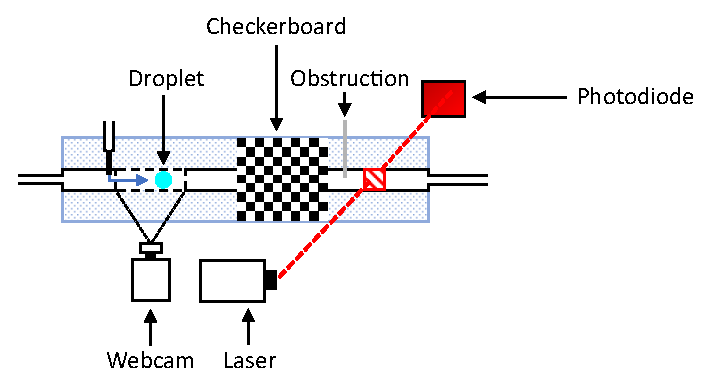
\includegraphics[scale=0.9]{Figures/Control.eps}
                    \caption{Figure to demonstrate the sealed chamber used to investigate continuously moving droplets. A cylindrical tunnel was created in a slide consisting of polydimethylsiloxane (PDMS). Droplets were injected through the top port and flowed from left to right. After photographing a calibration checkerboard with a webcam, a small slice of this tunnel was selected and continuously monitored, and the size of passing droplets determined. The droplet was then oscillated with a variety of methods, shown here as a small obstruction. Oscillations caused a laser beam directed at the tunnel to diffract, which was then detected with a photodiode.} 
                \label{fig:slide}
            \end{figure} 
    
        To move droplets through the slide, the 2 mm diameter capillary tubes were then connected to a fluid loop consisting of 3 mm diameter tubes. Mineral oil was used as a carrier medium to transport the spherical droplets. A t-junction was also placed at the return side of the loop to allow for simple bleeding of air. A t-junction was used because air was the least dense medium present, and as it moved to the highest point in the system, it pushed the oil and therefore the droplet, complicating analysis. After flowing through the system and being analysed in the slide, droplets were transported to a central reservoir. Here, as the droplets were of different density to the mineral oil, they would either sink or float and so they could be easily removed at a later point by hand using a syringe. To prevent these droplets from returning into the slide, the return and collection tubes were placed at different heights on opposite sides of the reservoir. A motor was used to transport the oil from the reservoir and around the loop. This setup is demonstrated in Figure \ref{fig:basic}.
        
            \begin{figure}[H]
                \centering                        
                    \hspace*{2.0cm}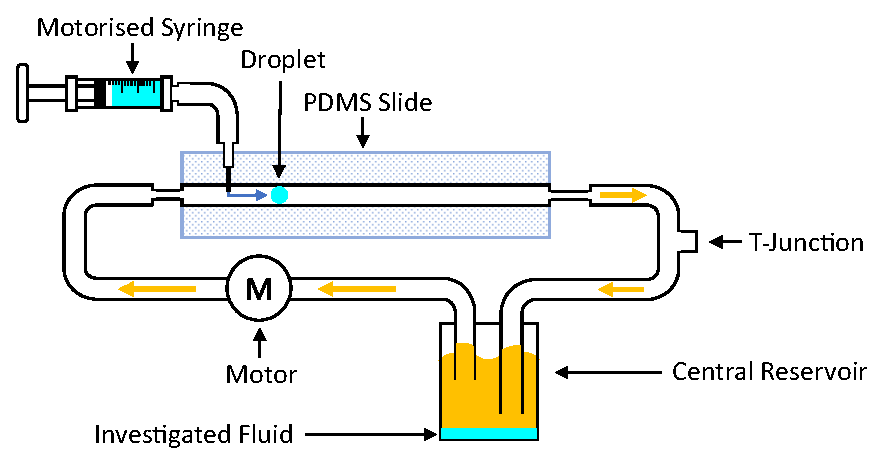
\includegraphics[scale=0.8]{Figures/Fluid.eps}
                    \caption{Figure to demonstrate the flow circuit used to investigate the rheological properties of droplets. Using a motor, a suspension fluid of mineral oil was transported from a central reservoir to a polydimethylsiloxane (PDMS) testing environment and back. A t-junction was placed in the return half of the loop to bleed air out of the system. A motorised syringe was used to suspend droplets of interest in the mineral oil that were subsequently analysed inside the PDMS slide. Droplets were then transported back to the reservoir, where they could be retrieved.}     
                \label{fig:basic}
            \end{figure} 

    \vspace*{-0.1cm}\subsection{Motor \& Syringe Pump\label{sect:method:motor}}

        To allow the speed of the fluid to be programmatically controlled, the motor was driven by a DAQ card. However, the available DAQ card lacked the circuitry to output sufficient current to drive the motor. Furthermore, the DAQ card had poor output resolution, making very fine control of fluid velocity impossible. A current boosting circuit was therefore produced, and is shown in Figure \ref{fig:MotorCircuit}.  
        
            \begin{figure}[H]
                \centering
                \hspace*{-1.3cm}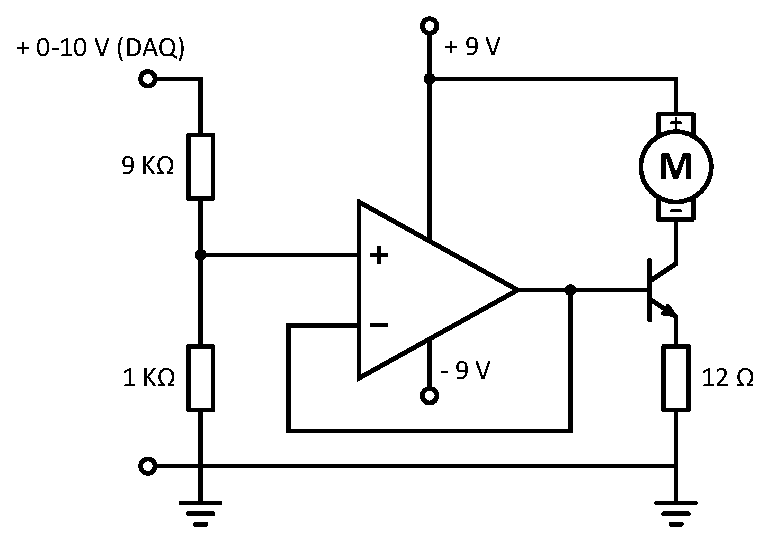
\includegraphics[scale=0.77]{Figures/MotorCircuit.eps}
                \caption{Figure showing the schematic of the circuit used to control the voltage applied to the motor programmatically. Depending on a 0 - 10 V input from a DAQ card, between 0 - 4 V could be output to the motor at 0 - 400 mA. This was required as the DAQ card alone was unable to produce sufficient current to drive the motor.}
                \label{fig:MotorCircuit}
            \end{figure}
        
        Depending on the 0 - 10 V inputted from the DAQ card, between 0 - 4 V was outputted to the motor through the power supply. This allowed the motor voltage to be more finely controlled. By powering the circuit with a current limited power supply, set at the maximum current rating of the motor, the motor could be driven at without being overloaded. The resistors were chosen both to provide the required output and to provide even heat dissipation across all components. Heat dissipation was further improved by attaching a heatsink to the transistor. The 12 $\Omega$ resistor was also replaced with three 36 $\Omega$ resistors\cite{artofelectronics} to reduce component stress on this section of the circuit. 
        
        To observe oscillations for the longest period of time possible the motor was run at 1.5 V. This was the lowest voltage that the motor could run at and hence, the slowest speed that the droplet could travel through the slide. By measuring the length of the slide and the time taken for a droplet to travel through the slide it was determined that the droplet travelled through the slide at 0.004 ms$^{-1}$.  
        
        Using a motorised syringe pump, it was also possible to produce droplets of a consistent size. Increasing the speed of the motor increased the size of droplets produced decreased and vice versa. Therefore, the size of the droplets produced was easily controlled by writing code to interface with the pump through a serial port and set it to run at set speeds. 
        
        
    \subsection{Determining Density\label{sect:method:density}}
    
        In previous experiments density, $\rho$, was typically calculated by using the radius, $R$, and mass, $m$, of each spherical droplet to determine its volume, $V$. The previous method of measuring the mass of the droplet was not viable in this project due to the closed nature of the system. In this project instead of measuring the density of each individual droplet, the density of the entire fluid was found. Measuring a larger volume of fluid resulted in a lower percentage error in the measurement of mass which improved the accuracy of the calculated density. By holding the fluid of interest in a syringe, the masses of an empty and filled syringe were easily compared with a measuring scale to determine the mass of the fluid. The corresponding volume was then easily determined from the scale of the syringe. 
        
    \subsection{Camera\label{sect:method:vision}}
        
        As the droplets in this project were not stationary, it was important that the programs written were efficient enough to analyse droplets before they exited the field of view of the camera. Furthermore, as MATLAB was an interpreted language and lacked hardware acceleration, webcam acquisition operated at very low frame rates. This made it difficult to track moving droplets in real time. This was overcome by using a package called Hebicam\cite{HebiCam}, which was initially created for streaming CCTV footage and was a MATLAB wrapper for the more efficient openCV\cite{opencv}. After adapting Hebicam for use with USB webcams, a 1080p video could be acquired at 30 FPS with spare processor overhead to perform calculations, as opposed to 6 FPS with none. To further improve the speed of calculations, images were not acquired in colour, but instead in grey-scale. This also reduced the size of stored data. A Logitech C920 webcam was chosen as it had high image quality, high resolution, and a wide field of view with which to view droplets. 
            
        One of the significant difficulties encountered during previous studies involved quickly computing the radius of droplets. Historically, authors have manually counted the width of droplets in pixels, before converting this to the real world distance $R$, using simple trigonometry and the focal length of the camera. These manual processes were used because using computer vision with transparent droplets was extremely difficult. This is despite the common requirement in manufacturing to identify droplets\cite{bubblegeneral}. Without perfect and even lighting surrounding droplets, no strong regions of contrast exist entirely around their boundary. As the droplets were transparent, their centres looked identical to their surroundings, confusing simple algorithms\cite{bubblegeneral}. Droplets could also have bright reflections in their middle, adding extra complexity. This was before considering the inevitable presence of noise in images. As a result of these factors, more complex algorithms take nearly a minute to run per frame, yet still only achieve detection accuracies of approximately 80\%\cite{bubble2}. In this project, these issues were overcome through the knowledge of the background of an image, along with the understanding of where the droplet was at any given time, and the assumption that it was spherical. 

        \subsubsection{Calibration\label{sect:method:vision:calib}}

            One of the major issues with only using the focal length of the camera to calculate $R$ was the incorrect assumption that images were perfectly planar. This was incorrect as non-linearities would be introduced into images by distortions such as fish-eye in the camera. To ensure that droplet size was calculated accurately, checkerboard calibration was therefore applied. This first involved taking multiple photographs of a square checkerboard of known checker size at multiple positions in the field of view of the camera. It was then possible to algorithmically determine various extrinsic properties of the camera, such as its optical centre, distortions, and skew\cite{CameraCalibration}, and use these to correct images. These distortions and subsequent corrections are illustrated in Figure \ref{fig:calibsetup}. 
                \begin{figure}[H]
                    \centering
                  \begin{subfigure}[b]{0.48\textwidth}
                        \hspace*{1.5cm} 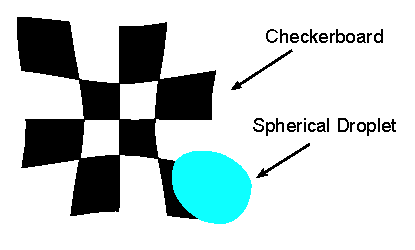
\includegraphics[width=\textwidth]{Figures/Distorted.eps}
                        \caption{Before Calibration}
                        \label{fig:calibsetup:distorted}
                    \end{subfigure}
                    \begin{subfigure}[b]{0.48\textwidth}
                        \hspace{1.8cm}
\includegraphics[scale=1.27]{Figures/Undistorted.eps}
                        \caption{After Calibration}
                        \label{fig:calibsetup:undistorted}
                    \end{subfigure}
                    \caption{Figure to illustrate the need to take into account lens distortions when determining the size of real world objects. Without calibration (a), distortions such as fish-eye caused objects to be warped, meaning that a spherical droplet did not appear to be spherical. By using a checkerboard with square checkers of known size, these distortions were found and accounted for (b). At this point, their size was more accurately calculated. }\label{fig:calibsetup}
                \end{figure}
                
             As additional calibration images increased calibration accuracy, 20 calibration images were taken in similar positions to those used during this project. The positions of the checkerboard in the calibration photos as determined by the algorithm are shown in Figure \ref{fig:calib}. 
            \vspace{0.5cm}
                \begin{figure}[H]
                    \centering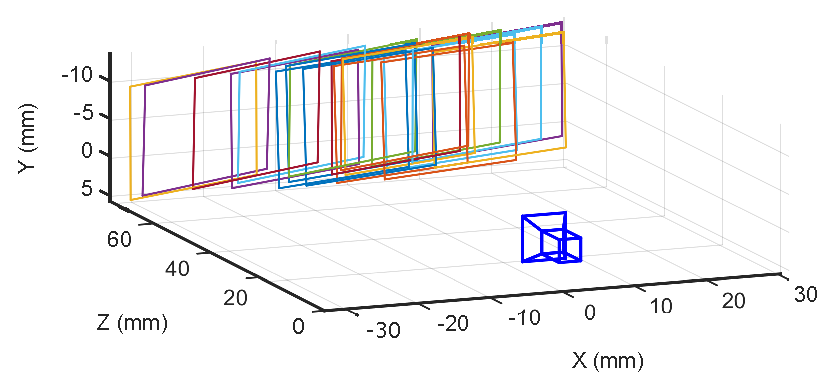
\includegraphics[scale=0.93]{Figures/CameraExtrinsics.eps}
                    \caption{Figure to demonstrate the multiple positions a checkerboard was placed in to calibrate a webcam. By taking multiple pictures of the checkerboard in multiple positions and knowing the size of the square checkers, the camera was algorithmically calibrated to reliably determine object size. As the positions of the checkerboard calculated by the algorithm agreed with the real-world placements, the camera was known to be accurately calibrated.}\label{fig:calib}
                \end{figure}
            
            \newpage After the camera was calibrated, $R$ could then be calculated by taking an image of a droplet and a checkerboard, as shown in Figure \ref{fig:slide}. The additional checkerboard was needed and had to be in plane with the droplet as the camera had no depth perception. Also, because the checkerboard did not move during the experiment, the checkerboard only had to be imaged once during each run of the experiment. This negated the need to calculate lens distortions after each droplet was observed, greatly improving efficiency. 
            
            The size of the checkers in the checkerboard were also considered. Larger checkers had a lower percentage error from imperfect focusing, but smaller checkers could be placed in greater numbers. However, there was a limitation in that the slide that the checkerboard was mounted on was of a finite size. To determine the optimum checkerboard size for this project, the camera was calibrated with checkers between 0.10 and 1.00 mm in size. Circles of known radius between were then printed, and their size determined. Ultimately, it was found that checkers of size 0.20 x 0.20 mm in a 10 x 11 grid gave the most accurate results. 
            
            There was an added complication to this process in that the PDMS used to create the slide was not perfectly flat. As the algorithms worked on the assumptions that checkerboard was flat and the droplet was in plane with the checkerboard, significant errors would have been introduced if the checkerboard was glued to this uneven surface. The pattern was therefore instead printed on a long piece of paper and tensioned to the back of the slide. However, this resulted in a small 1 mm disparity in depth between the droplet and the checkerboard, resulting in a small error. Using simple trigonometry to measure the distance to the droplets, this error was calculated to result in a 0.05 mm underestimation of all values of $R$, and as such was added to all calculated values of $R$. 
        
        \subsubsection{Determining Droplet Size\label{sect:method:vision:size}}
                
            After calibrating the camera, $R$ was then determined by first taking a photograph of the droplet. However, this was not possible while the droplet was moving. This was because photographs would suffer from motion blur, and the droplets were slightly stretched while in motion. As such, the motor had to be stopped before taking a photograph. This was done by continuously checking for the presence of a droplet in the slide. As the droplets were confined to a small area at any one time, only a small 3 mm long window of the slide was ever observed at one time to improve performance. The motor could, therefore, be stopped when a droplet was present within this small window.    
                
            To determine if a droplet was present, a background photo of the window was first taken with oil flowing but without a droplet. After turning on the pump to make a droplet, every time a frame of video was captured, the window was subtracted from the corresponding background. Non-black pixels, therefore, corresponded to differences between the two photos. To increase the contrast of these differences, the contrast was multiplied by the arbitrarily selected log(6) which increased the signal-to-noise ratio in the image. When a droplet was present in the window, fully bright regions could be easily seen in the area where the droplet was. Once an arbitrary threshold of bright pixels was reached, the droplet was confirmed as being in the window, and the motor stopped. These steps are demonstrated in Figure \ref{fig:detector}.
            
                    \begin{figure}[H]
                        \centering
                        \begin{subfigure}[b]{0.3\textwidth}
                            
\includegraphics[width=\textwidth]{Figures/DropFinder/DropFinder1.eps}
                            \caption{Background}
                            \label{fig:detector:back}
                        \end{subfigure}
                        ~ 
                        \begin{subfigure}[b]{0.3\textwidth}
                            
\includegraphics[width=\textwidth]{Figures/DropFinder/DropFinder2.eps}
                            \caption{Foreground}
                            \label{fig:detector:fore}
                        \end{subfigure}
                        ~ 
                        \begin{subfigure}[b]{0.3\textwidth}
                            
\includegraphics[width=\textwidth]{Figures/DropFinder/DropFinder3.eps}
                            \caption{Difference}
                            \label{fig:detector:diff}
                        \end{subfigure}
                        \caption{Figure to demonstrate how droplets were detected after being created by a mechanical pump. A region of the webcam was defined, and a background image taken (a). The region was then continuously monitored. If a droplet was present in the region (b), it could be detected by calculating the difference between (b) and (a) and multiplying by log(6). If enough bright pixels were observed (c), a droplet was known to be present in the system.}\label{fig:detector}
                    \end{figure}
            
            After stopping the motor, $R$ could then be calculated. A new photo was first taken of the droplet, which was now guaranteed to be in the pre-defined window, and its outline calculated. This was achieved with a 5-stage algorithm. Firstly, background detail was removed as before by subtracting the image from the background. To bring out fine dark detail and reduce bright noise, a top-hat filter was then used to set all pixels with brightnesses below 10 to 0 (i.e. black), and all pixels with brightnesses above 20 to 255 (i.e. white). Of the remaining data, an automatic binarising algorithm was then applied to bring out fine detail further and form a solid white horseshoe. This horseshoe was then turned into a convex hull and filled in. This shape was then detected with a Circular Hough Transform based algorithm\cite{imfindcircles} as the droplet was known to be smaller than the capillary length and therefore, spherical. Each stage of this algorithm is shown in Figure \ref{fig:size}.
            \vspace{0.5cm}
                \begin{figure}[H]
                    \centering
                    \begin{subfigure}[b]{0.3\textwidth}
                        
\includegraphics[width=\textwidth]{Figures/SizeFinder/SizeFinder1.eps}
                        \caption{Raw Image}
                        \label{fig:size:1}
                    \end{subfigure}
                    ~ 
                    \begin{subfigure}[b]{0.3\textwidth}
                        
\includegraphics[width=\textwidth]{Figures/SizeFinder/SizeFinder2.eps}
                        \caption{Background Subtraction}
                        \label{fig:size:2}
                    \end{subfigure}
                    ~ 
                    \begin{subfigure}[b]{0.3\textwidth}
                        
\includegraphics[width=\textwidth]{Figures/SizeFinder/SizeFinder3.eps}
                        \caption{Top Hat}
                        \label{fig:size:3}
                    \end{subfigure}
                
                    \begin{subfigure}[b]{0.3\textwidth}
                        
\includegraphics[width=\textwidth]{Figures/SizeFinder/SizeFinder4.eps}
                        \caption{Binarise}
                        \label{fig:size:4}
                    \end{subfigure}
                    ~ 
                    \begin{subfigure}[b]{0.3\textwidth}
                        
\includegraphics[width=\textwidth]{Figures/SizeFinder/SizeFinder5.eps}
                        \caption{Convex Hull}
                        \label{fig:size:5}
                    \end{subfigure}
                    ~  
                    \begin{subfigure}[b]{0.3\textwidth}
                        
\includegraphics[width=\textwidth]{Figures/SizeFinder/SizeFinder6.eps}
                        \caption{Detected Circle}
                        \label{fig:size:6}
                    \end{subfigure}
                    \caption{Figure to demonstrate the method in which a bounding box could be drawn around a droplet to determine its size. After photographing the droplet (a), the photo could be subtracted from an image taken just before the droplet was present (b). A top hat filter was then applied to this droplet to remove noise (c), before thresholding to extract fine detail (d). The largest remaining horseshoe-shape could then be turned into a solid convex hull (e). As the droplet was assumed to be spherical, the bounding box of the droplet could then be found with a simple Circular Hough Transform (f).}\label{fig:size}
                \end{figure}
            
            After determining the boundary of the droplet, the boundary points were corrected for camera distortions using calibration produced by the checkerboard. A box of size $D_x$ x $D_y$ was then drawn around the remaining shape, pixels converted to mm using the fixed checkerboard, and Equation \ref{eq:radii} used to determine the droplet radius. Once the size of the droplet was determined, the motor was re-engaged to transport the droplet to the laser so that it could be analysed using the laser and photodiode.
    
    \subsection{Oscillating Droplets\label{sect:method:oscillating}}
        
        After determining the size of the droplets, their vibrational spectra had to be determined. It was not possible to follow previous authors and induce vibrations with compressed air\cite{Temperton2012,Sharp2011} as the droplets were contained in a closed system. Magnetic coils were also considered, however, this would have limited the materials that could be investigated in the future. Although the 30 FPS camera recording did not give enough data points to calculate the spectra of an oscillating droplet, it was sufficient to observe oscillations clearly. Oscillations were therefore confirmed to present if they could be observed by eye.
        
        To induce oscillations, multiple methods were attempted. The first of these methods included the use of piezoelectric actuators and asymmetrically weighted vibration motors to vibrate the droplet. Secondly, the speed of the motor was changed to pulse rapidly to perturb the droplet using the control circuitry shown in Figure \ref{fig:MotorCircuit}. 
        
        A high voltage DC electric field was also considered. For reasons not thoroughly understood, it had been shown that a short, high voltage DC pulse passed across an unpolarised droplet can cause it to oscillate\cite{DCfield}. As such, two exposed wires were dug into the PDMS on either side of the fluid channel, and each wire connected to either side of a 6 kV power supply to set up a simple circuit. As PDMS has a high breakdown voltage of\cite{PDMSBreakdown} 6 kV mm$^{-1}$, the electric field would be highly localised and directly through the channel, causing moving droplets to be given a sharp impulse. To maximise the strength of the electric field, the wires were dug into the PDMS as close to the fluid channel as possible. This allowed the power supply to be left on at all times, which was necessary as no equipment was available to switch the supply rapidly on and off. 
        
        The final method in which oscillations were induced, was to place a copper wire slightly inside the channel. This method relied on the water having a high surface tension of around 70 mNm$^{-1}$, which was much higher than mineral oil at 30 mNm$^{-1}$. Water based droplets, amongst others, would, therefore, be inclined to cling to a new surface when brought nearby. As the mineral oil had a much lower surface tension, it would not. As the droplet was moving, its equilibrium state would eventually change back to being spherical. It would then "ping" back, thus inducing oscillations. 
        
    \subsection{Laser \& Photodiode\label{sect:method:laser}}
    
        Although previous investigations found lower resonant frequencies\cite{Temperton2012}, the 30 FPS webcam was found to be too slow to capture enough data to perform calculations with. To detect oscillations, a photodiode was instead used to capture the intensity fluctuations of a laser as it was refracted through the droplet. This setup is shown in Figure \ref{fig:slide}, with the laser on one side of the slide and the photodiode on the other. As the droplets in this project could be assumed to have had a different refractive index to that of the carrier oil\cite{viscosity1,viscosity2}, it followed that the presence of a droplet along the laser would cause laser light to be scattered differently. Furthermore, as the shape of droplets varied as they oscillated, they caused light to scatter in proportion to their degree of oscillation. 
        
        As droplets would be moving as they oscillated, the laser was broadly focused on a wide area of the slide to increase the amount of time the oscillating droplet was within the laser, thus providing more data. However, the laser was brightest about its centre, and so the system was more sensitive around this region than others. To increase the area of this region of high sensitivity, the solid angle of this bright region was increased by placing the laser at a glancing angle of over 45$^{\circ}$ to the slide, instead of being face on. To further improve this situation, the laser was later replaced with a wider, more powerful He-Ne laser.
        
        \newpage To amplify the output of the photodiode to measurable values, a simple amplification circuit was created\cite{artofelectronics}. A schematic is shown in Figure \ref{fig:PDCircuit}. A variable resistor was used to act as a gain controller, allowing the output voltage to be made as high as possible within the 0 - 10 V recording range of the DAQ card, increasing sensitivity. A 220 pF capacitor was not originally included but was later added to reduce noise\cite{artofelectronics}. A larger capacitor was considered, as it would reduce more noise. However, it made the circuit less sensitive to small changes. To prevent 50 Hz noise from an AC-DC power supply, the laser was instead driven by batteries.
    
            \begin{figure}[H]
                \centering
                \hspace{0.1cm}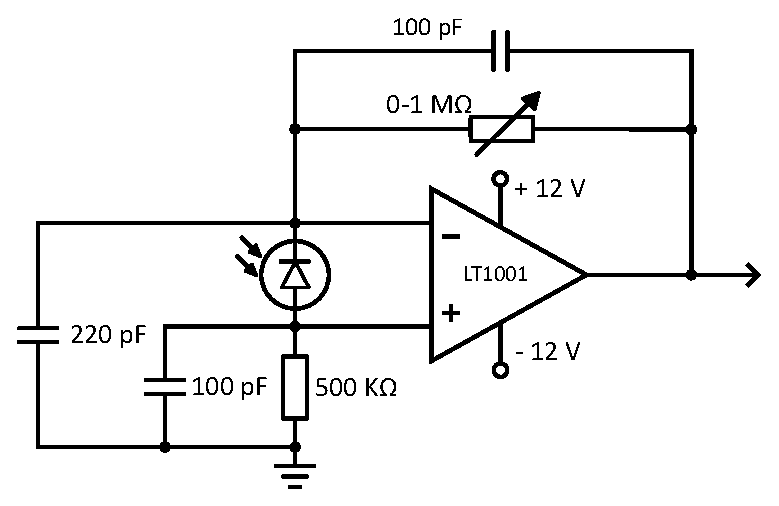
\includegraphics[scale=0.8]{Figures/PDCircuit.eps}
                \caption{Figure showing a schematic of the circuit used to amplify the reading of the photodiode used in this project. Based on the laser light incident on the photodiode a voltage was output between 0 - 10 V which was read using the DAQ card. Extra smoothing is applied in the form of a 220 pF capacitor, and amplification gain is set by the resistance of a 1 M$\Omega$ variable resistor.}
                \label{fig:PDCircuit}
            \end{figure}
    

    \subsection{Running Experiments\label{sect:method:exp}}
        
        Using a user-friendly toolbox, which required minimum setup, droplets were rapidly analysed. To set up the code and control the equipment, files and folders were first automatically created to store raw data. At this point, a previous camera calibration could be selected, or a new one created with a selected number of images. After approving this calibration, operating parameters such as motor voltage and photodiode recording time were then defined. The DAQ card, pump and webcam were then interfaced with so they could be controlled. At this point, the camera was imaged, the checkerboard found, and camera extrinsics calculated. The window (area) of the webcam image in which the droplet was to be imaged was then selected. These setup steps are shown in Figure \ref{fig:setup:flow}.
        
            \newpage
            \begin{figure}[H]
                \centering
                \hspace*{-5.4cm}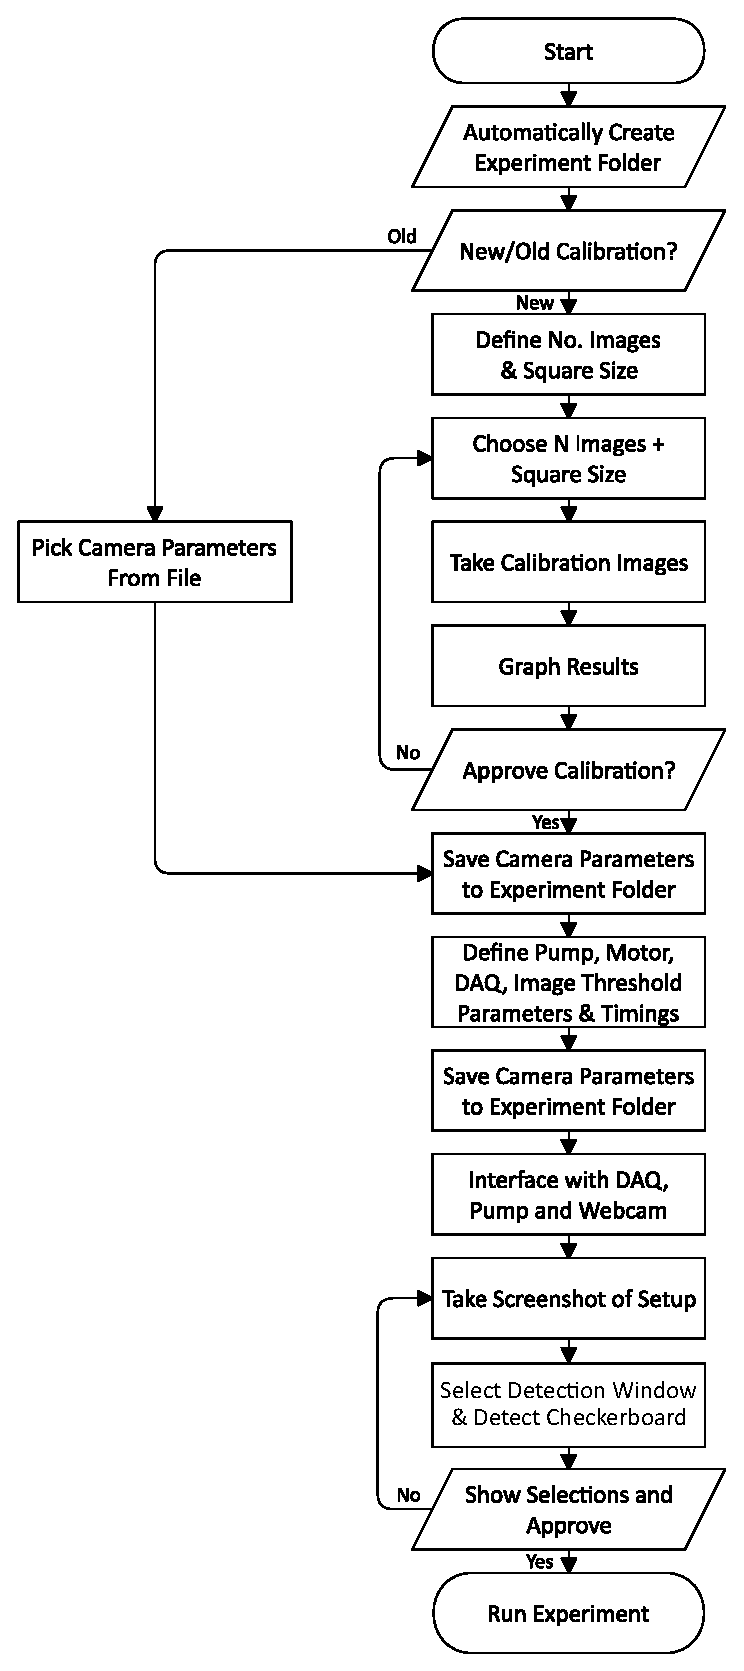
\includegraphics[scale=0.8]{Figures/FlowSetup.eps}
                \caption{Figure showing a flow chart demonstrating the process by which the system was set up to allow for the automated measuring of rheological properties of droplets.}
                \label{fig:setup:flow}
            \end{figure}
            
        \newpage From here, no further user input was required, and experiments were automatically run. As shown in Figure \ref{fig:setup:logic}, this first began with turning on the motor and running it for a few seconds to clear out any stray material from the slide. The detection window defined earlier was then imaged, and the background image shown in Figure \ref{fig:detector:back} taken. The syringe pump was then turned on for just long enough to produce a single droplet of a consistent size. A video was then taken of the window in real time, and after every frame, the foreground was subtracted from the background and compared. Once the threshold conditions described in Section \ref{sect:method:vision:size} were met, the motor was stopped, distortions accounted for, and the size of the droplet found. The motor was then re-engaged, and the photodiode spectrum recorded. After a pre-defined amount of time, oscillations were detected in this spectrum by looking for significant changes in the signal, and this area Fourier transformed. The Fourier transform could then be calculated, along with $f$ and $\Delta f$. This data was then saved to disk. Extra droplets could then be produced to produce further results, which were averaged together to calculate final values of $\eta$ and $\gamma$. All code has been included as supplementary material.
    
            \vspace{0.5cm}\begin{figure}[H]
                \centering
                \hspace*{-1cm}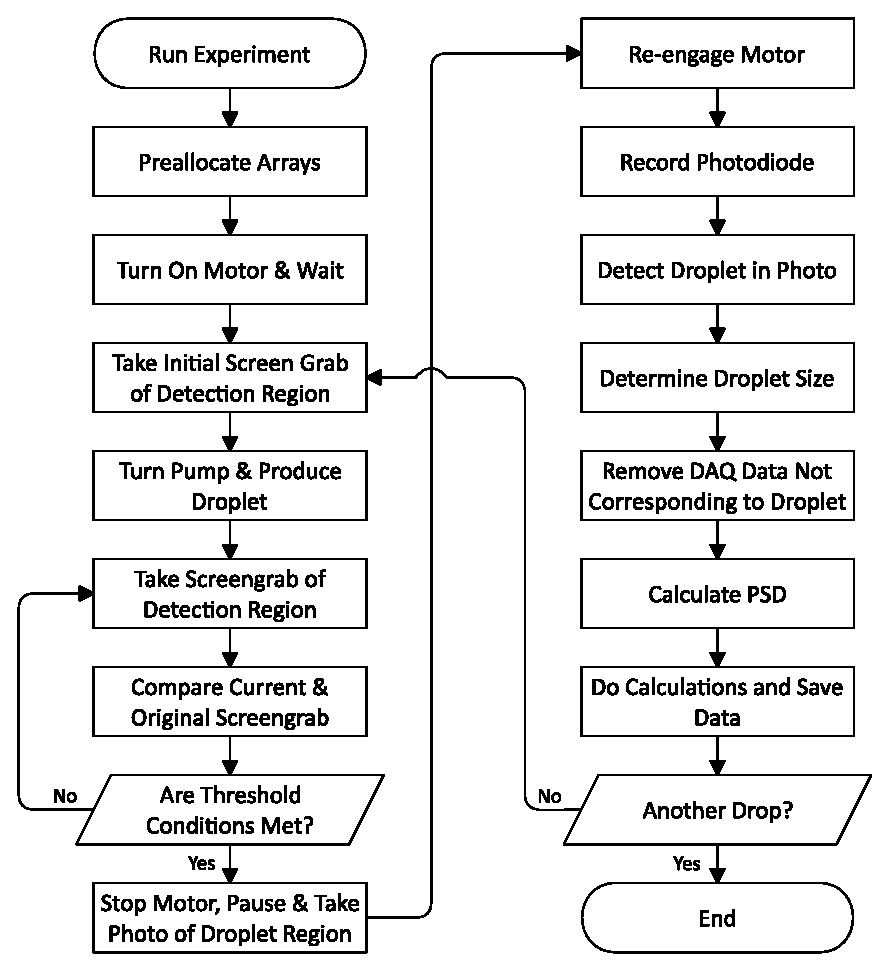
\includegraphics[scale=0.8]{Figures/FlowLogic.eps}
                \caption{Figure showing a flow chart to demonstrate the control logic used by the system to automatically measure the rheological properties of droplets.}
                \label{fig:setup:logic}
            \end{figure}

\section{Error Analysis\label{sect:error}} 
    
    There were several major sources of error in the project. When calculating the mass of the liquid, an error was produced when comparing the difference in mass between a filled and empty syringe. As such, the precision of the measuring scale, 0.001 g, was added in quadrature with itself. There was also an error on the volume of the syringe, which was defined as the precision of the scale, 0.2 mL. These two errors were propagated together to determine the error on the density of the droplet.
    
    Furthermore, there were several sources of error involved when calculating $R$. Firstly, there was the mean error of 0.41 $\pm$ 0.02 pixels across the 20 calibration images when calibrating the camera, which produced an error when converting between pixel space and real space. However, as the bounding box finding algorithm only operated to a per-pixel accuracy, this sub-pixel error was negligible. This was seen when calculating the size of known objects, which was found to have an average standard deviation of 0.03 mm away from the expected size. This is shown in Figure \ref{fig:calib:error}. 
        
            \begin{figure}[H]
                \centering
                \hspace*{-1cm}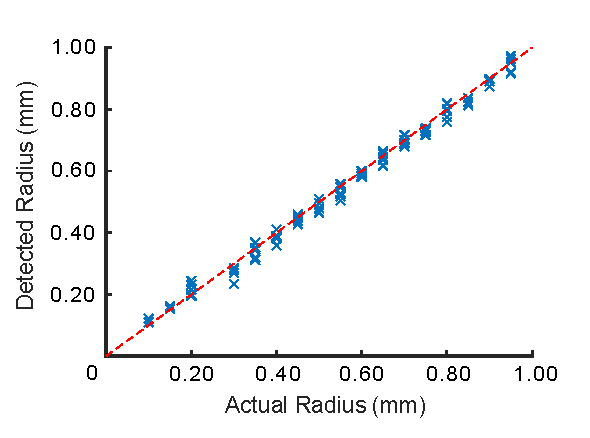
\includegraphics{Figures/CameraCalib.eps}
                \caption{Figure to demonstrate the accuracy by which a calibrated webcam could calculate the radius of multiple bright circles of known size. Given the small standard deviation of 0.03 mm from expected values and strong linear agreement across multiple radii, it can be seen that the calibration and size calculation algorithms used in the project worked as intended.}
                \label{fig:calib:error}
            \end{figure}
    
    Additionally, there was also an error due to the imperfect finding of the bounding boxes around the droplet. By comparing the bounding boxes of 20 droplets drawn by hand and by the algorithm, 100\% of the droplets were detected by the algorithm to within $\pm$ 2 pixels in radius. As the droplets had diameters of around 80 pixels, it was estimated that the boundary of a droplet could be calculated to within a 5\% error. 5\% of $R$ was therefore added in quadrature with the 0.03 mm discussed above to calculate the final error on $R$. 
    
    The errors on $f$ and $\Delta f$ were also considered. The error on $f$ was defined as the resolution of the frequency axis of the Fourier transformed signal. The error on $\Delta f$ was similarly defined as the error on $f$ added in quadrature with itself. The errors on $\rho$, $R$, $f$ and $\Delta f$ were then propagated through Equations \ref{eq:SurfaceTension} and \ref{eq:Viscosity} to calculate the errors on $\eta$ and $\gamma$ for each run of the experiment. These errors were found by adding the standard deviation of all calculated values of $\eta$ and $\gamma$ in quadrature, with the standard deviation of all of the errors calculated for each value of $\eta$ and $\gamma$.
    
    Ultimately, the largest source of error in Equations \ref{eq:SurfaceTension} and \ref{eq:Viscosity} was considered to be the small amount of time that oscillations could be recorded for. This was because frequency resolution was a function of both sampling rate and sample time, but sampling rate could not be reliably increased past 3,000 Hz without causing equipment errors. As such, the lowest possible frequency resolution was set by the time that oscillations could be detected for. As discussed below, oscillations could often only be detected for 0.5 seconds. In these cases, the frequency resolution would be as low as 2 - 3 Hz, or approximately 30\% of the observed value of $f$. Furthermore, as Equations \ref{eq:SurfaceTension} and \ref{eq:Viscosity} were both a second order function of $f$ and $\Delta f$, substantial errors were produced. 
    
\section{Results \& Discussion\label{sect:results}}

    \subsection{Water in Air\label{sect:results:WaterInAir}}
     
    To determine the expected frequency about which droplets would oscillate, a single sessile water droplet was analysed. After determining that, for the water used in this experiment, $\rho =$ 990 $\pm$ 33 kgm$^{-3}$, the droplet was blown on to give it the impulse needed to start oscillating. Although this was not ideal, only an approximate value was desired to guide later results. It can be seen from Figure \ref{fig:Water} that this produced clear oscillations for approximately 2.5 seconds. This indicated that oscillations observed in this project would be visible for no longer than this, as the droplets in oil would not only be moving but also be damped by the surrounding oil. 
 
            \begin{figure}[H]
            \centering
                    \begin{subfigure}[b]{0.48\textwidth} \hspace*{-0.2cm}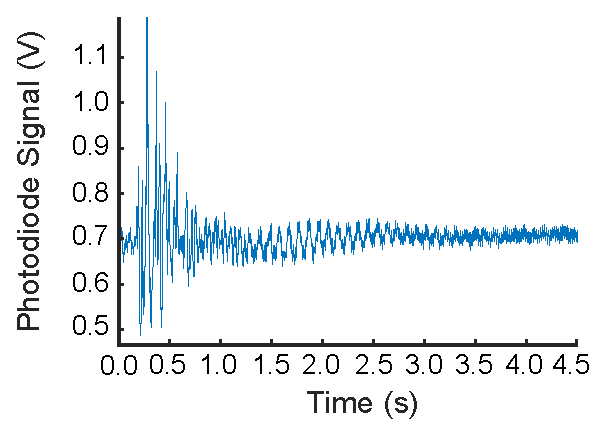
\includegraphics[width=\textwidth]{Figures/WaterSignal.eps}
                    \caption{Photodiode Signal}
                    \label{fig:Water:Signal}
                \end{subfigure}\hspace{3pt}
                \begin{subfigure}[b]{0.48\textwidth}
                    \hspace*{0.2cm}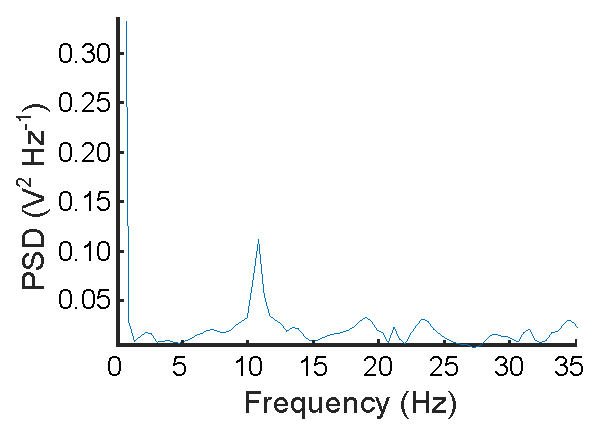
\includegraphics[width=\textwidth]{Figures/WaterSignalPD.eps}
                    \caption{Fourier Transform}
                    \label{fig:Water:FT}
                \end{subfigure}
            \caption{Figure to demonstrate the original signal obtained from the photodiode (a), and the resulting Fourier transform (b) of a sessile droplet in air vibrated by blowing on it. It can be seen that this produced clear oscillations for approximately 2.5 seconds at a frequency around 10 Hz. }\label{fig:Water}
            \end{figure} 
            
    Once the photodiode signal was Fourier transformed it was observed that the oscillations were at a frequency of approximately 10 Hz. As such, droplets of water in oil were therefore expected to oscillate at similar frequencies. The change in medium and size was not expected to change $f$ by more than a few Hz owing to Equations \ref{eq:SurfaceTension} and \ref{eq:Viscosity}. This experiment also confirmed that the Fourier transform was working as expected as this gave very similar results to the results found by Temperton et al\cite{temperton}. This was because the $n = 1$ and $n = 2$ peaks could be clearly observed in Figure \ref{fig:Water:FT}, and the graphs were of similar form to Figure \ref{fig:temperton}.

    \subsection{Control Equipment\label{sect:results:control}}
    
        The equipment used in this project was also tested to check it was working as expected. As can be seen in Figure \ref{fig:MotorCalib}, the motor voltage increased linearly with the voltage output through the DAQ card. As expected, using DAQ voltages of 0 - 10 V, voltages of 0 - 4 V were output by the circuit. Furthermore, as a current limiting power supply was used, once the DAQ voltage increased above 6.4 V, increasing the DAQ voltage further did not increase the motor voltage above 4 V, preventing damage to the motor. As expected, lowering the DAQ voltage lowered the driving speed of the motor without any spikes in voltage.
        
        \begin{figure}[H]
            \centering
            \hspace*{-1cm}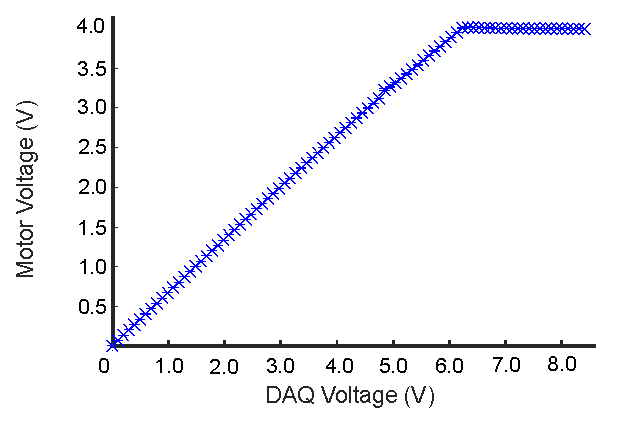
\includegraphics{Figures/MotorCalib.eps}
            \caption{Figure to demonstrate that the output voltage provided to a motor by a current boosting circuit, depends on its input voltage. A current limiter was also attached to prevent overvolting the motor. The circuit was created to allow a 2 - 4 V, 200 - 400 mA motor to be programmatically driven by a 0 - 10 V DAQ card without the capability to output current. As the circuit outputs the correct voltages and currents until the clearly visible current limit, the circuit can be considered to be working correctly.}\label{fig:MotorCalib}
        \end{figure}
        
        It was also found that the size of droplets could be accurately calculated, as there was a strong agreement between expected and detected circle sizes. This is shown in Figure \ref{fig:calib:error}. However, the algorithm struggled to detect circles under a radius of 0.30 mm, and hence, there was a lower limit to the size of the droplets that could be analysed in this project.
        
        
    \subsection{Oscillating Droplets\label{sect:results:oscillation}}
      
        Initially, the use of piezoelectric actuators and asymmetrically weighted vibration motors were considered to oscillate the droplets. However, these had to be attached externally to the slide and therefore made the slide as a whole vibrate and not only the droplet within as desired. Hence, any oscillations of the droplets were not detectable.
        
        Next, an attempt was made to induce oscillations by changing the speed of the motor using the control circuitry shown in Figure \ref{fig:MotorCircuit}. Although the motor could have been pulsed rapidly, this was akin to driving the droplets at a single frequency, rather than applying an impulse. This was confirmed by the presence of a single peak in the power spectral density at the pulse frequency of the motor. Instead, oscillations were attempted to be induced by applying one sudden change in motor voltage, with the hope of having the sudden change in velocity cause the droplet to stretch horizontally and therefore induce oscillations. This was unsuccessful as the force applied by the change of velocity was too weak to induce any observable oscillations.
        
        At this point, a DC electric field was used to oscillate the droplets. However, it can be seen from Figure \ref{fig:control} that there was a significant amount of noise produced when the power supply for the electric field voltage was on. This was because the standard deviation of the photodiode signal was directly proportional to the voltage produced by the supply. It could, therefore, be concluded that the source of the noise was the high voltage power supply, and was likely to be due to stray magnetic fields being produced. Although oscillations could be visibly observed with the DC electric field, they could not be measured as a result of the noise. Footage of these oscillations was included in the supplementary material.
        
        \begin{figure}[H]
            \centering
            \hspace*{-1.2cm}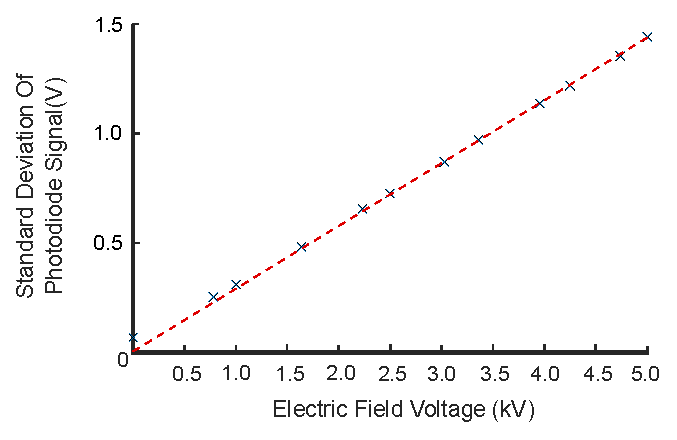
\includegraphics[scale=0.95]{Figures/ElecFieldNoise.eps}
            \caption{Figure to demonstrate the noise produced in a photodiode circuit by the presence of a high voltage power supply. As there is a linear relationship, the noise is clearly due to the high voltage power supply along with the wires. This noise was the reason why the electric field could not be used to observe oscillations.}     
            \label{fig:control}
        \end{figure} 
        
        \vspace*{-0.3cm}To reduce the stray magnetic fields produced in the wires causing interference in the photodiode circuit, by Lenz's law, all wires were tightly twisted in pairs. The photodiode circuit was also remade to fit in a small grounded metal box. Although this decreased noise significantly, the noise was still too large to observe oscillations. This was because the amplitude of the late timescale oscillations could be as low as 0.2 V and because an electric field voltage of over 3.0 kV was needed to see any visible oscillations, the noise from the power supply swamped the signal. Therefore the use of a DC electric field was therefore not a viable option for this project. 
        
        Finally, a wire obstruction was pushed into the slide. This is shown in Figure \ref{fig:slide}. Starting from a sharp "ping" when the droplet detached from the needle, oscillations were clearly observed. Footage was been included in the supplementary material to demonstrate this. This is shown in Figure \ref{fig:oscillation}. Although an exponential decay should have been present in an oscillatory signal, its absence was easily understood. As the laser was not uniform, the amplitude of the signal due to the oscillations of the droplet was found to be dependent on the position of the droplet within the laser beam. When qualitatively comparing this typical signal with the expected signal from Figure \ref{fig:temperton:signal}, both signals had similar shapes and timescales. This demonstrated that the observed signal was an oscillation. 
        
         \vspace{0.2cm}\begin{figure}[H]
            \centering   
            \begin{subfigure}[b]{0.48\textwidth}
                \hspace*{0cm}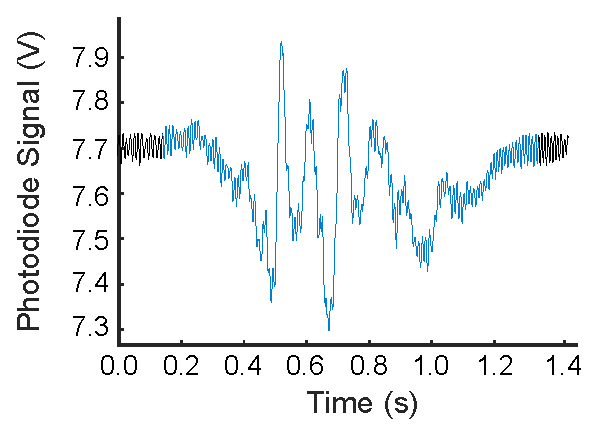
\includegraphics[width=\textwidth]{Figures/PingSignal.eps}
                \caption{Photodiode Signal}
                \label{fig:oscillation:signal}
            \end{subfigure}\hspace{3pt}
            \begin{subfigure}[b]{0.48\textwidth}
                \hspace*{0.1cm}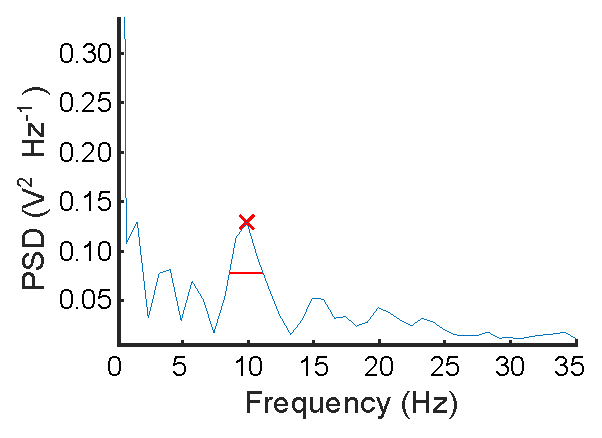
\includegraphics[width=\textwidth]{Figures/PingPD.eps}
                \caption{Fourier Transform}
                \label{fig:oscillation:FT}
                \end{subfigure}
            \caption{Figure to demonstrate an oscillation obtained in this project for a water droplet suspended in oil (a), and the resulting Fourier transform (b). It can be seen that oscillations were observed for around one second demonstrated by the blue section of the photodiode signal. Both this Fourier transform, and the expected Fourier transform from Figure \ref{fig:temperton:PD} had similar shapes and timescales. This demonstrated that the observed signal was an oscillation. The observed frequency of around 10 Hz is shown by the red cross, and the detected full-width-half-maximum is shown by the red line. }\label{fig:oscillation}
        \end{figure} 
        
        After Fourier transforming this signal, a significant peak was observed at a frequency around the 10 Hz that was expected. Furthermore, the peak was Lorentzian in shape. This was in agreement with the expected value from Figure \ref{fig:Water:FT}, giving further evidence that the signal acquired was indeed due to oscillations. It was therefore concluded that moving droplets could be oscillated using an obstruction.
        
        It can also be seen in Figure \ref{fig:oscillation:signal} that the algorithm for determining the section of the photodiode signal when oscillations were present was also clearly successful. This is shown in this figure as the blue section of the signal. It can also be seen in Figure \ref{fig:oscillation:FT} that the algorithm for determining the frequency of oscillation, represented by the red cross, and the full-width-half-maximum, represented by the red line, also worked as intended.
        
        However, when using the high speed camera, it was observed that the oscillations induced by an obstruction were of a lower magnitude and a shorter timescale to those created with the DC electric field. To obtain the signal graphed above, several adjustments had to be made. To increase the strength of the "ping" (and therefore the oscillatory signal), the droplet had to be made to cling more strongly to the obstruction. In an attempt to do this, the obstruction material was first considered. A syringe needle, nickel plated wire, and copper plated wire were tested, and it was found that the most consistent results were seen with the copper plated wire. The obstruction was also roughed up with sandpaper to increase its surface area. A polarising charge was then introduced to the obstruction by oxidising it. A Van-der-Graff generator was also considered to polarise the obstruction, increasing attraction strength further. However, applying a strong charge when the droplet was nearby caused the droplet to break apart. The height of the obstruction with respect to the amplitude of oscillations was also considered. When the obstruction was deeper into the channel, droplets broke up more easily, while shallower obstructions resulted in oscillations of lower magnitude. The obstruction was therefore placed two thirds of the way into the tunnel. 
        
    \subsection{Multiple Droplet Investigations\label{sect:results:multi}}
    
        At this point, ten droplets were analysed in the system, and the average values of both the surface tension, $\gamma$, and viscosity, $\eta$, calculated. Ultimately, it was found that $\gamma$ = 21.54 $\pm$ 17.57 mNm$^{-1}$ and $\eta$ = 11.77 $\pm$ 6.63 x 10$^{-4}$ Nm$^{2}$s$^{-1}$. Although $\eta$ was within one standard deviation of its expected value\cite{expected2} of 8.94 x 10$^{-4}$ Nm$^{2}$s$^{-1}$, $\gamma$ was only within two standard deviations of its expected value\cite{expected1} of 72.80 mNm$^{-1}$. Although they were still within an order of magnitude of their expected values, investigations in air routinely achieved far greater accuracy to decimal place precision. However, the calculated values were likely to be more accurate when considering the fact that the equations and expected values used were for water in air, and not water in oil. Furthermore, they were likely to be correct, as all droplets were calculated to have oscillated between 5 - 15 Hz, which was in line with the 10 Hz expected. 
        
        This analysis was also made significantly more complicated by the extremely large errors on $\gamma$ and $\eta$. This is clearly seen in the large vertical errors in Figure \ref{fig:finalresults}. As discussed in Section \ref{sect:error}, this was mostly due to the low signal time of 0.5 seconds, resulting in large errors on $f$. This was because the frequency step in a Fourier transform depended on both the time of the signal being transformed and the sampling rate of this signal. Although the DAQ card could theoretically sample beyond the 3,000 Hz used in experiments, various errors occurred when attempting to do so. This large error on $f$ can be clearly observed in Figures \ref{fig:vsgamma:f} and \ref{fig:vseta:f} through the large horizontal error bars. 
    
        \begin{figure}[H]
            \centering   
            \begin{subfigure}[b]{0.48\textwidth}
                \hspace*{-0.2cm}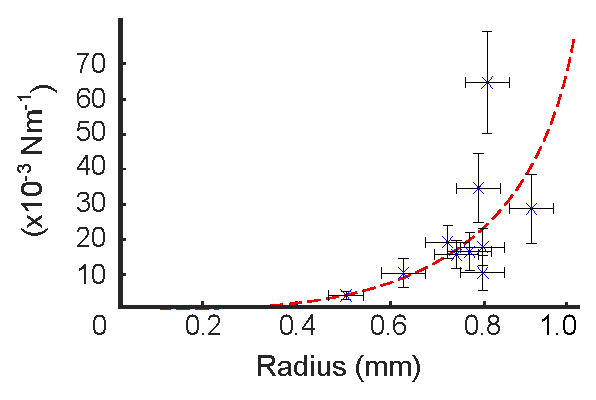
\includegraphics[width=\textwidth]{Figures/r_vs_gamma.eps}
                \caption{Radius vs Surface Tension}
                \label{fig:vsgamma:r}
            \end{subfigure}\hspace{3pt}
            \begin{subfigure}[b]{0.48\textwidth}
                \hspace*{0.2cm}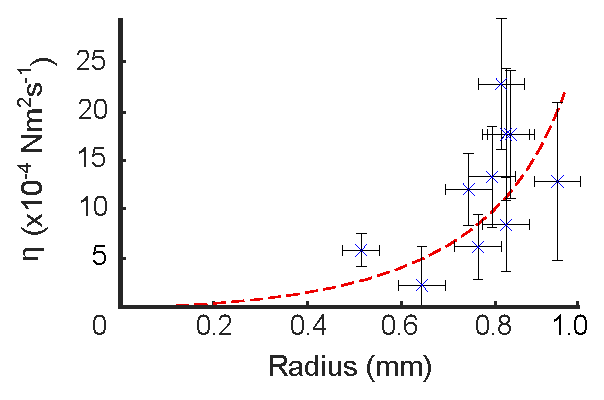
\includegraphics[width=\textwidth]{Figures/r_vs_eta.eps} 
                \caption{Radius vs Viscosity}
                \label{fig:vseta:r}
                \end{subfigure}
                ~
            \begin{subfigure}[b]{0.48\textwidth}
                \hspace*{-0.2cm}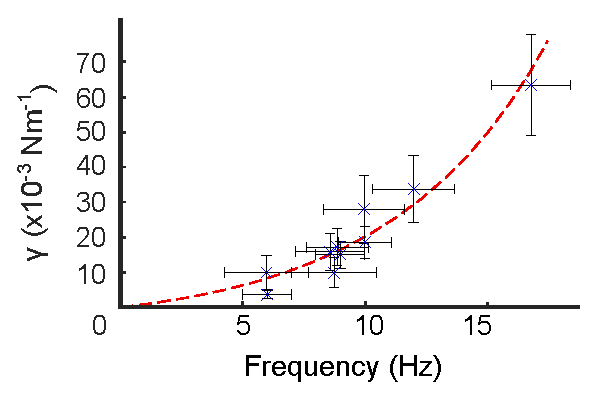
\includegraphics[width=\textwidth]{Figures/f_vs_gamma.eps}
                \caption{Frequency vs Surface Tension}
                \label{fig:vsgamma:f}
            \end{subfigure}\hspace{3pt}
            \begin{subfigure}[b]{0.48\textwidth}
                \hspace*{0.2cm}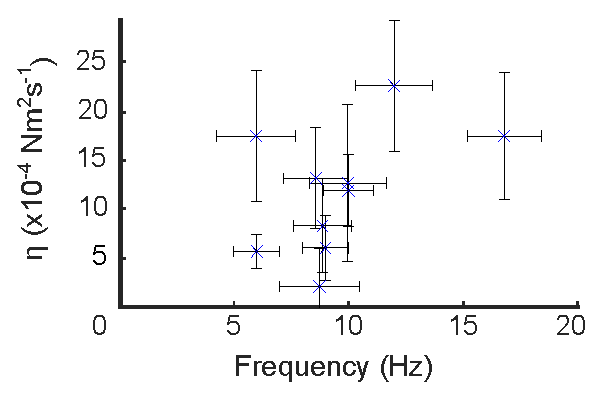
\includegraphics[width=\textwidth]{Figures/f_vs_eta.eps} 
                \caption{Frequency vs Viscosity}
                \label{fig:vseta:f}
                \end{subfigure}
            \caption{Figure to demonstrate the results found during an experiment to investigate the rheological properties of water. It was found in (a) and (b) that the average surface tension, $\gamma$ = 21.54 $\pm$ 17.57 mNm$^{-1}$, and in (c) and (d) that the average viscosity, $\eta$ = 11.77 $\pm$ 6.63 x 10$^{-4}$ Nm$^{2}$s$^{-1}$. Despite the large errors, there were clear positive trends with the exception of (d) between $\eta$ and $\gamma$ with respect to the calculated values of radius and oscillatory frequency. However, these trends were unexpected, as flat horizontal lines should have been seen about $\gamma$ = 72.80 mNm and $\eta$ = 8.94 x 10$^{-4}$ Nm$^{2}$s$^{-1}$.}
            \label{fig:finalresults}
        \end{figure} 
        
        \vspace*{-0.4cm}
        The low sampling rate may have also caused a significant shift in the calculated values, regardless of errors. Through simulation, Egry et al.\cite{egry} demonstrated that $\gamma$ could be incorrect by up to a factor of 5 if only a very small number of data points were taken. Furthermore, this factor increases with increasing sample rate. As their sampling rate was significantly lower than the sampling rate used in this project, the error on $\gamma$ was likely to be greater than a factor of 5.
        
        Another major source of error seen in Figure \ref{fig:finalresults} was that the data did not fall on a horizontal straight line. As $\eta$ and $\gamma$ were intrinsic to the material investigated, they should be expected to remain constant, regardless of any value measured to determine them. As such, the line of best fit for Figures \ref{fig:vsgamma:r} and \ref{fig:vsgamma:f} should have been a horizontal line at 72.80 mNm$^{-1}$, while the line of best fit for Figures \ref{fig:vseta:r} and \ref{fig:vseta:f} should have been a horizontal line at 8.94 x 10$^{-4}$ Nm$^{2}$s$^{-1}$. Instead, there was a clear and significant positive trend between measured values of $R$ or $f$ and $\eta$ or $\gamma$. This indicated that the issue might not have been due to flawed data collection methods, but instead due to incomplete equations and theory. A more thorough development of the underlying theory is therefore critical to future success.
        
        Although this general trend could be clearly observed, it was not possible to discern any clear line of best fit from these graphs, as the large scatter and large errors made fitting a line of best fit a very subjective process. However, with the exception of Figure \ref{fig:vseta:f}, the lines of best fit could potentially be seen as exponential in nature. Given that the decays in oscillations were exponential, and the mineral oil acted to damp the droplet oscillations, this seemed to provide further evidence that Equations \ref{eq:SurfaceTension} and \ref{eq:Viscosity} did not completely apply to the case of liquid in a damped medium.
        
        \newpage Furthermore, the droplets were not perfectly spherical, especially when moving. This is easily observed in Figure \ref{fig:detector:diff}. As discussed in Section \ref{sect:lit}, if a droplet was not spherical its vibrational spectra would be altered in non-linear fashions. However, this non-linearity has yet to be derived\cite{harrold2}. Furthermore, Egry et al.\cite{egry} also found that if the droplets rotated, there would be a significant shift in $f$, dependant on the axis of rotation. Because the channel created was formed from a mould, the inevitable imperfections would have altered the flow of the oil, causing droplets to rotate. This may have acted slightly differently on droplets of different size, introducing a non-linearity on the extent that the $f$ was shifted. This may further explain the non-linearities observed. Further non-linearities may have also been caused by droplets oscillating at amplitudes greater than 0.1$R$, as amplitude could not be precisely controlled.
        
        Additionally, it was found that $R$ did not scale with $f$ as expected. It was expected that smaller droplets with smaller $R$ would vibrate at higher values of $f$. However, as shown in Figure \ref{fig:rvsf}, this was not the case. Instead, it could be seen that as $R$ decreased, so too did $f$, even when taking errors into account. Besides droplets not being spherical, this could be explained by the rotation of the droplets, as above. Such rotations could have been caused by the channel not being perfectly smooth. However, it could not be determined if droplets were indeed rotating without a more sophisticated camera setup. In future, the presence of rotations should be tested for, and if confirmed the subsequent shift in $f$ should be taken into account through the use of the equations described by Egry\cite{egry}. 
        
        \vspace{0.5cm}\begin{figure}[H]
            \centering
            \hspace*{-0.7cm}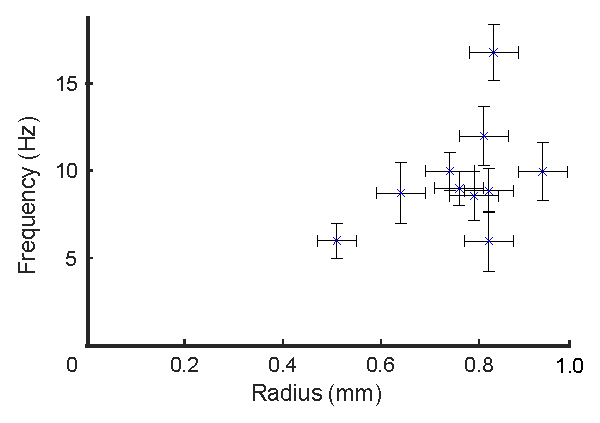
\includegraphics{Figures/r_vs_f.eps}
            \caption{Figure to demonstrate the dependence on the frequency of droplet oscillation and the radius of the droplet. It can be seen that $R$ did not scale with $f$ as expected. It was expected that smaller droplets with smaller $R$ would vibrate at higher values of $f$. Instead, it could be seen that as $R$ decreased, so too did $f$, even when taking errors into account.}     
            \label{fig:rvsf}
        \end{figure} 
        
        
\newpage \section{Limitations \& Future Improvements\label{sect:limitations}}
    
    There were numerous limitations with the investigation. Firstly, the motorised syringe pump had to be interfaced with over a COM port. This had a significant delay, reducing the throughput of droplets in the fluidic system. Furthermore, once the syringe pump began to be turned, it could not be stopped, often resulting in stray droplets being produced if the initial pump parameters were not set correctly. These stray droplets often passed through the laser at the same time as the droplet being investigated, producing extra signals. As all data from these runs of the experiment had to be discarded, this partly explains why few results were obtained. In the future, a more modern controller with the ability to turn off the motorised syringe pump once a droplet was detected in the system should be used.
    
    There were also a few drawbacks to the droplet finding algorithms used. When detecting droplets, as shown in Figure \ref{fig:detector}, the algorithm was highly sensitive. As such, it would incorrectly trigger and erroneously detect a droplet if the oil was cloudy or had impurities. In future, an object finding algorithm could be employed instead of the arbitrary thresholds used here, provided it ran efficiently. Because the droplets were faint, it would also fail to trigger unless a dark object was placed behind it to increase background contrast. Instead, the need to track droplets in real time with a camera could be entirely negated by using another laser and photodiode to act as a "trip" switch. When a droplet is present, there would be a rapid change in the photodiode signal. The motor could then be stopped, and the droplet imaged as before.
    
    The camera used also had several limitations. When measuring $R$, errors were largely due to the pixel-level precision and the small number of pixels taken up by the droplet. Furthermore, the top-hat filter demonstrated in Figure \ref{fig:size:3} was also very arbitrary in its setup, and had to be tweaked for different lighting conditions. As the droplets produced for the experiment were typically around 40 pixels in radius, they only took up 2,000 of the 2,073,600 pixels in a 1920 x 1080 image, or only around 0.25\% of the pixels. This was wasteful. It also meant that the circle finding algorithm struggled with droplets with a radius below 0.3 mm, limiting the range of droplet sizes that could be investigated. If the camera had a lower focal length, it could be positioned far closer to the droplet, allowing droplets to take up a higher percentage of the pixels in the image, resulting in more effective image detection. This would also result in a significantly smaller error when determining $R$. Alternatively, a higher resolution camera would also increase the accuracy of boundary detection due to the larger number of pixels detected in the droplet. However, this would come at the expense of computational efficiency due to the larger number of pixels. 
    
    One of the major difficulties encountered when investigating moving droplets involved short signal times. As oscillations could only be observed when a droplet was oscillating in the path of the laser beam, the effectiveness of the system was highly dependant on the alignment of the laser and the obstruction. This extreme sensitivity meant that moving the laser by only 2 mm was sufficient to render any oscillation completely unrecordable. This was the main reason why only ten results were obtained and why optimising obstruction material, obstruction height, laser angle and laser position could only be achieved qualitatively. 
    
    There were multiple methods by which this could be improved. For example, the laser could be defocussed to increase its width. Although this was attempted, it was only viable to a small extent as the intensity of the beam quickly became too weak to be detected by the photodiode. As such, the beam could instead be reshaped horizontally by refracting it through a bi-convex lens. Although this was also attempted by placing a glass rod next to the slide, the horizontally shaped beam was not intense enough to yield a high enough photodiode signal. In the future, a wide array of multiple photodiodes could be used to capture more light. While a more sensitive avalanche photodiode would also be an improvement, this comes with the caveat that any laser used must be highly stable. A more powerful laser would also be a potential improvement. Alternatively, the low oscillation time could be improved upon through the use of a slower motor. It would also be possible to extend the computer vision code to completely stop a droplet once it began oscillating. 
    
    Alternatively, the detection of oscillations could be made more rigorous by replacing the laser with a high speed camera. This is because a laser and photodiode only produce a single value over time, whilst a camera would produce multiple points in each image to calculate with. In this case, oscillations could be calculated by considering the variation of droplet diameter over time. This could be further enhanced by calculating diameters at multiple angles through the droplet. This approach would both increase sensitivity and make noise less problematic. Furthermore, droplets could be tracked over the entire length of the slide, as opposed to only over the diameter of the laser beam. This approach is also suggested by multiple authors, such as Egry et al.\cite{egry}, who have used simple implementations of this method to great effect.
    
    Furthermore, the recordable timescales of oscillations appeared to decrease significantly during the experiment. Although oscillatory signals were visible for 1.0 - 1.5 seconds early on in the project, later oscillations, despite improvements made to the setup, were only visible for less than 0.5 seconds. This may have been due to decreasing performance of the photodiode. Although the noise due to the photodiode circuit did not change, the photodiode may have become less sensitive, meaning that only the strongest oscillations were visible. This could not be quantitatively investigated by comparing signal amplitude because of the high sensitivity and variable gain of the photodiode circuit. 
    
    As it was found that droplets could be oscillated through both obstructions and electric fields, future work should focus around refining methods to observe these oscillations. In particular, work should focus on observing oscillations induced by DC electric fields, as stray magnetic fields prevented their further investigation in this project. Following on from the previous limitations, issues due to stray fields could be negated by replacing the laser with a high speed camera. Furthermore, high speed, high voltage switching equipment could be used to switch off the electric field when recording oscillations. 
    
    Numerous other small improvements could be made. One of the reasons a high-throughput fluidic system was developed was so that droplets could be analysed using a non destructive technique. However, due to time constraints a method to reliably extract the droplets from the oil after analysis was not developed beyond using a syringe. This system was not developed in this project, as a large reservoir of oil was used and the water being investigated was not rare or expensive. Hence, future studies could develop a system to extract the droplets to allow them to be recycled through the system.
    
\vspace*{-0.2cm}    
\section{Conclusions\label{sect:conc}}

    In summary, it was successfully demonstrated that the rheological properties of droplets can be determined in a self-contained system. This involved the creation of both hardware and software to automatically produce single droplets of fluid inside a sealed PDMS slide. The PDMS was later improved upon with a perspex slide. The droplets were then suspended in mineral oil. To transport the droplets through this system, a motor was attached, and control circuitry produced to drive it at low speed. The practicality of this circuit was also verified. Through the use of checkerboards and computer vision algorithms, a webcam was calibrated and the radius of every droplet calculated in real time to $\pm$ 0.05 mm accuracy. 
    
    Using the assumption that suspended droplets would be spherical, the theory was discussed by which the viscosity, $\eta$, and surface tension, $\gamma$, of the droplets could be determined. Oscillations were induced in the droplets at their resonant frequencies by applying an impulse. These were subsequently detected by firing a laser at an angle to the oscillating droplet and detecting this laser with an amplified photodiode. Various methods were considered for inducing oscillations. Piezoelectric actuators and asymmetrically weighted vibration motors were found not to induce oscillations. High voltage DC electric fields were found to induce oscillations but caused significant noise in the control circuitry, making this a non-viable method. Results were, however, obtained for an obstruction of oxidised, sandpapered copper wire. Due to oscillatory signals being highly sensitive with respect to the alignment of the laser, the obstruction material and height could only be investigated qualitatively. 
    
    After manually determining that water droplets should oscillate at approximately 10 Hz, the automated system was used to determine $\eta$ and $\gamma$ for multiple droplets. By investigating ten droplets with a radius of 0.5 - 1.0 mm radius, all were found to oscillate between 5 - 15 Hz. After averaging, it was calculated that $\gamma$ = 21.54 $\pm$ 17.57 mNm$^{-1}$ and $\eta$ = 11.77 $\pm$ 6.63 x 10$^{-4}$ Nm$^{2}$s$^{-1}$. Although $\eta$ was within one standard deviation of its expected value of \cite{expected2} 8.94 x 10$^{-4}$ Nm$^{2}$s$^{-1}$, $\gamma$ was only within two standard deviations of its expected value of\cite{expected1} 72.80 mNm$^{-1}$.
    
    However, there were multiple major explanations for these discrepancies. Firstly, the equations used to calculate $\eta$ and $\gamma$ only applied to water in air, and not water in oil based experiments. This introduced errors as additional damping mechanisms were present. Furthermore, the droplets were not perfectly spherical when moving. As this was a core assumption of the equations used, describing the dynamics of the system would require additional non-linear terms. As such, a complete understanding of the associated theory is needed before forming a complete analysis in the future, and droplets should be stopped in place when observing oscillations. The large error-bars on $\eta$ and $\gamma$ were mainly due to the short times that oscillations could be detected for. These were likely due to a combination of the damping effects of oil and the extremely high sensitivity between the signal length and the alignment of the laser. These issues may have also been compounded by the photodiode decreasing in sensitivity over time. 
    
    As such, there are numerous major improvements that could be made in the future. For one, the camera could be replaced for one with a shorter focal length and brought much closer to the droplet. A bi-convex lens could also be used to spread the laser beam horizontally, and detected with a horizontal array of photodiodes. Alternatively, the DC electric field, which gave far greater oscillation amplitudes, could be used by turning off the power supply with high speed switching equipment. This would resolve the issue seen with noise. Further, the laser and photodiode could be replaced with a high speed camera and improved lighting conditions, with the variation of droplet diameter over time used as the time dependent signal from which to calculate frequencies. This could be further enhanced by calculating diameters at multiple angles through the droplet. 

    Ultimately, this investigation and final results are sufficient to demonstrate a proof of concept of a method to investigate droplets in a closed high-throughput system. Although the errors produced were large and final values were only within an order of magnitude from the expected values, they can be primarily explained by low signal times and incomplete theory for moving inviscid droplets. Besides improvements to theory, future experimentation should focus on replacing the laser with a low focal length, high speed camera, and implementing a switchable high voltage DC field. From the foundations laid in this project, it is evident that the vibration of droplets in automated high throughput systems could be a key method for rheology in the future.
    

% -----------
% REFERENCES
% -----------
\newpage
\bibliographystyle{unsrtnat}
\bibliography{references}

% -----------
% CODE
% -----------
\newpage
\appendix{}
\section{Code}
    \subsection{Camera Calibration}
        \lstinputlisting{Code/getCalib.m}
        \lstinputlisting{Code/CameraCalib.m}
        
    \newpage\subsection{Automated Controller}
        \lstinputlisting{Code/Auto_System_2.m}

% -----------
% FIN
% -----------
\end{document}    